\documentclass[12pt]{article}

\usepackage{parskip,amsthm,amsmath,amsfonts,amssymb}
\usepackage{multicol,cancel}
\usepackage[shortlabels]{enumitem}
\usepackage[letterpaper,margin=1in,bottom=0.7in]{geometry}
\newcommand{\dd}[2]{\dfrac{d #1}{d #2}}
\newcommand{\ddd}[2]{\dfrac{d^2 #1}{d #2^2}}
\newcommand{\pd}[2]{\dfrac{\partial #1}{\partial #2}}
\newcommand{\ppd}[2]{\dfrac{\partial^2 #1}{\partial #2^2}}
\newcommand{\ppdd}[3]{\dfrac{\partial^2 #1}{\partial #2\partial #3}}
\newcommand{\brf}[2]{\left(\frac{#1}{#2}\right)}
                       % Bracket-frac, e.g. for (n\pi x/L) in Fourier series
\newcommand{\fsin}[1]{\sin\brf{#1 \pi x}{L}}
\newcommand{\fcos}[1]{\cos\brf{#1 \pi x}{L}}
\newcommand{\fsint}[1]{\sin\brf{#1 \pi t}{L}}
\newcommand{\fcost}[1]{\cos\brf{#1 \pi t}{L}}
\newcommand{\RR}{\mathbf{R}}
\newcommand{\CC}{\mathbf{C}}
\newcommand{\ZZ}{\mathbf{Z}}
\newcommand{\mks}[1]{\begin{flushright}(#1 marks)\end{flushright}}

\usepackage{tikz}
\newcommand{\lapl}[6]{
\begin{tikzpicture}[scale=2]
  \draw (0,0) -- (0,1);
  \draw (0,1) -- (1,1);
  \draw (1,1) -- (1,0);
  \draw (1,0) -- (0,0);
  \node at (0.5,0.5) {$#6$};
  \node [below] at (0.5,0) {$#1(x,0)=#2$};
  \node [above] at (0.5,1) {$#1(x,\pi)=#3$};
  \node [left] at (0,0.5) {$#1(0,y)=#4$};
  \node [right] at (1,0.5) {$#1(\pi,y)=#5$};
\end{tikzpicture}
}

\newcommand{\onelapl}[6]{
\begin{tikzpicture}[scale=2]
  \draw (0,0) -- (0,1);
  \draw (0,1) -- (1,1);
  \draw (1,1) -- (1,0);
  \draw (1,0) -- (0,0);
  \node at (0.5,0.5) {#6};
  \node [below] at (0.5,0) {$#1(x,0)=#2$};
  \node [above] at (0.5,1) {$#1(x,1)=#3$};
  \node [left] at (0,0.5) {$#1(0,y)=#4$};
  \node [right] at (1,0.5) {$#1(1,y)=#5$};
\end{tikzpicture}
}


\newcommand{\mlapl}[6]{
\begin{tikzpicture}[scale=2]
  \draw (0,0) -- (0,1);
  \draw (0,1) -- (1,1);
  \draw (1,1) -- (1,0);
  \draw (1,0) -- (0,0);
  \node at (0.5,0.5) {#1};
  \node [below] at (0.5,0) {$#6(x,0)=#2$};
  \node [above] at (0.5,1) {$#6(x,\pi)=#3$};
  \node [left] at (0,0.5) {$#6(0,y)=#4$};
  \node [right] at (1,0.5) {$#6(\pi,y)=#5$};
\end{tikzpicture}
}
\newcommand{\laplneu}[6]{
\begin{tikzpicture}[scale=2]
  \draw (0,0) -- (0,1);
  \draw (0,1) -- (1,1);
  \draw (1,1) -- (1,0);
  \draw (1,0) -- (0,0);
  \node at (0.5,0.5) {#6};
  \node [below] at (0.5,0) {$#1(x,0)=#2$};
  \node [above] at (0.5,1) {$#1(x,\pi)=#3$};
  \node [left] at (0,0.5) {$\partial_x#1(0,y)=#4$};
  \node [right] at (1,0.5) {$\partial_x#1(\pi,y)=#5$};
\end{tikzpicture}
}

\theoremstyle{remark}
\newtheorem{rmk}{Remark}

\theoremstyle{definition}
\newtheorem{question}{Question}
\newtheorem{answer}{Answer}


%%%%%%%%%%%%%%%%%% Add extra space before theorems

\begingroup 
\makeatletter 
\@for\theoremstyle:=definition,remark,plain,TheoremNum\do{% 
\expandafter\g@addto@macro\csname th@\theoremstyle\endcsname{% 
\addtolength\thm@preskip\parskip 
}% 
} 
\endgroup 


\title{Methods 3 - Question Sheet 8}
\author{J. Evans}
\date{}

\begin{document}
\maketitle


\begin{question}(10 marks)\\
Solve the wave equation $\partial_t^2\phi=\partial_x^2\phi$ with the initial conditions
\begin{enumerate}[(a)]
\item * $\phi(x,0)=x\qquad\partial_t\phi(x,0)=x^2$.
\item $\phi(x,0)=x^2\qquad\partial_t\phi(x,0)=x$.
\item $\phi(x,0)=0\qquad\partial_t\phi(x,0)=k\sin kx$.
\item * $\phi(x,0)=\begin{cases}
0 & \mbox{ if }|x|>1\\
1 & \mbox{ if }|x|\leq 1,
\end{cases}\qquad\partial_t\phi(x,0)=\begin{cases}
0 & \mbox{ if }|x|>1\\
-1 & \mbox{ if }|x|\leq 1.
\end{cases}$
\end{enumerate}
In this last case illustrate your answer with a spacetime diagram.
\end{question}

\begin{answer}
We know that the general D'Alembert solution to the wave equation is a function $\phi(x,t)$ of the form
\[\phi(x,t)=F(x+t)+G(x-t).\]
We use this in what follows.
\mks{1}
\begin{enumerate}[(a)]
\item * The initial conditions give us
\[\phi(x,0)=F(x)+G(x)=x,\qquad\partial_t\phi(x,0)=F'(x)-G'(x)=x^2.\]
Integrating the second of these gives
\[F(x)-G(x)=x^3/3+C\]
(we will see soon that the constant can be ignored) so solving for $F(x)$ gives us
\[F(x)=G(x)+C+x^3/3=-G(x)+x\]
which implies
\[G(x)=\frac{1}{2}(x-x^3/3-C)\]
which in turn implies
\[F(x)=x-\frac{1}{2}(x-x^3/3-C)=\frac{1}{2}(x+x^3/3+C)\]
so $F(x+t)+G(x-t)=\frac{1}{2}(x+t+(x+t)^3/3)+\frac{1}{2}(x-t-(x-t)^3/3)$ (the constants cancel out as mentioned earlier).
\mks{3}
\item  The initial conditions give us
\[\phi(x,0)=F(x)+G(x)=x^2,\qquad\partial_t\phi(x,0)=F'(x)-G'(x)=x.\]
Integrating the second of these gives
\[F(x)-G(x)=x^2/2+C\]
(we will see soon that the constant can be ignored) so solving for $F(x)$ gives us
\[F(x)=G(x)+C+x^2/2=-G(x)+x^2\]
which implies
\[G(x)=\frac{1}{2}(x^2/2-C)\]
which in turn implies
\[F(x)=x^2-\frac{1}{2}(x^2/2-C)=\frac{1}{2}(3x^2/2+C)\]
so $F(x+t)+G(x-t)=\frac{3}{4}(x+t)^2+\frac{1}{4}(x-t)^2$ (the constants cancel out as mentioned earlier).
\item The initial conditions give us
\[\phi(x,0)=F(x)+G(x)=0,\qquad\partial_t\phi(x,0)=F'(x)-G'(x)=k\sin kx.\]
Integrating the second of these gives
\[F(x)-G(x)=-\cos kx+C\]
(we will see soon that the constant can be ignored). Since the first equation gives $F(x)=-G(x)$, the second becomes
\[2F(x)=-\cos kx+C=-2G(x)\]
so $F(x+t)+G(x-t)=\frac{1}{2}\cos(k(x-t))-\frac{1}{2}\cos(k(x+t))$ (the constants cancel out as mentioned earlier).
\item * The initial conditions give us
\begin{align*}
\phi(x,0)&=F(x)+G(x)=\begin{cases}
0&\mbox{ if }x<-1,x>1\\
1&\mbox{ if }-1\leq x\leq 1
\end{cases},\\
\partial_t\phi(x,0)&=F'(x)-G'(x)=\begin{cases}
0&\mbox{ if }x<-1,x>1\\
-1&\mbox{ if }-1\leq x\leq 1
\end{cases}.\end{align*}
Integrating the second of these gives
\[F(x)-G(x)=\begin{cases}
0&\mbox{ if }x<-1\\
-1-x&\mbox{ if }-1\leq x\leq 1\\
-2&\mbox{ if }x>1.
\end{cases}\]
(ignoring constants) so solving for $F(x)$ and $G(x)$ gives us
\begin{align*}
2F(x)&=\begin{cases}
0&\mbox{ if }x<-1\\
-x&\mbox{ if }-1\leq x\leq 1\\
-2&\mbox{ if }x>1.
\end{cases},\\
2G(x)&=\begin{cases}
0&\mbox{ if }x<-1\\
2+x&\mbox{ if }-1\leq x\leq 1\\
2&\mbox{ if }x>1.
\end{cases}
\end{align*}
i.e.
\begin{align*}
F(x+t)&=\begin{cases}0&\mbox{ if }x+t<-1\\
-(x+t)/2&\mbox{ if }x+t\in[-1,1]\\
-1&\mbox{ if }x+t>1
\end{cases}\\
G(x-t)&=\begin{cases}0&\mbox{ if }x-t<-1\\
1+(x-t)/2&\mbox{ if }x-t\in[-1,1]\\
1&\mbox{ if }x-t>1
\end{cases}\\
\end{align*}
\mks{4}
The resulting function is best illustrated by a plot:
\mks{2}
\begin{center}
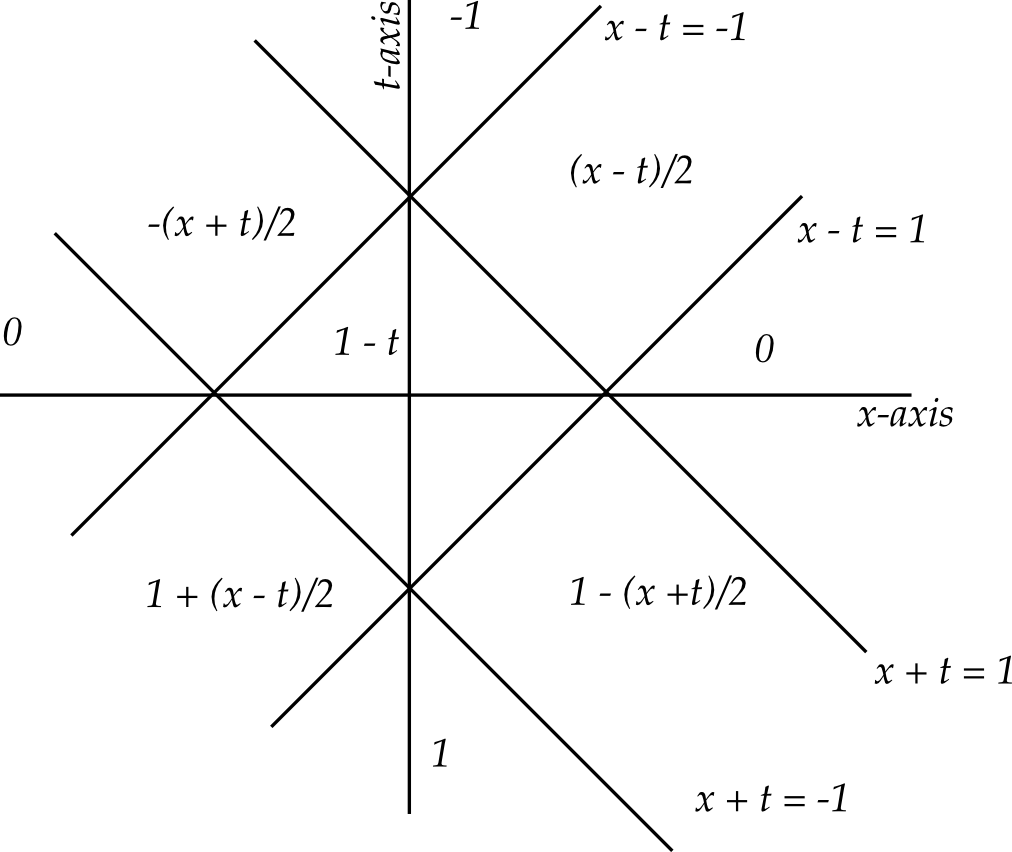
\includegraphics{qun-sh7-1d.png}
\end{center}
\end{enumerate}
\end{answer}
\newpage

\bigskip

\begin{question}(10 marks for * parts)\\
For each of the following equations:
\begin{enumerate}[(i)]
\item * Find coordinates $u,v$ such that the left-hand side of the equation becomes $\partial_u\partial_vF$.
\item * Find the general solution of the equation.
\item * Find the particular solution for the given initial conditions.
\end{enumerate}
\begin{enumerate}[(a)]
\item * $F_{xx}+5F_{xy}+6F_{yy}=0$, $F(x,0)=\sin(x)$, $\partial_yF(x,0)=\cos(x)$.
\item * $2F_{xx}+3F_{xy}+F_{yy}=x$, $F(x,0)=x$, $\partial_yF(x,0)=0$.
\item $F_{xy}+F_{yy}=\sin x$, $F(x,0)=x$, $\partial_yF(x,0)=x$.
\end{enumerate}
\end{question}

\begin{answer}
In each case we use the proposition in the notes which says that if $\alpha$ and $\beta$ are the roots of $AT^2+BT+C=0$ then under the change of coordinates $x=s+t$ and $y=-\beta s-\alpha t$ the operator $A\partial_x^2+B\partial_x\partial_y+C\partial_y^2$ becomes $A\partial_s\partial_t$.
\mks{1}
\begin{enumerate}[(a)]
\item * In this case we have $A=1$, $B=5$ and $C=6$. The roots are $\alpha=-2$ and $\beta=-3$ so the coordinates we desire are $s,t$ where $x=s+t$ and $y=2s+3t$, so $t=y-2x$ and $s=3x-y$. The equation is now $F_{st}=0$ with general solution $M(t)+N(s)=M(y-2x)+N(3x-y)$ for arbitrary functions $M$ and $N$.
\mks{2}
The initial conditions now give
\[M(-2x)+N(3x)=\sin x,\qquad M'(-2x)-N'(3x)=\cos x\]
so integrating the second gives $-M(2x)/2-N(3x)/3=\sin x$ therefore solving these simultaneous equations for $M$ and $N$ we get $M(-2x)=-8\sin(x)$ and $N(3x)=9\sin x$, so $M(u)=8\sin(u/2)$ and $N(u)=9\sin(u/3)$ which gives
\mks{3}
\[F(x,y)=8\sin((y-2x)/2)+9\sin((3x-y)/3)\]
It is always a good idea to check that the final $F$ does indeed satisfy the initial conditions (this one does).
\item * In this case we have $A=2$, $B=3$ and $C=1$. The roots are $\beta=-1$ and $\alpha=-1/2$ so the coordinates we desire are $s,t$ where $x=s+t$ and $y=s+t/2$, so $t=2x-2y$ and $s=2y-x$. The equation is now $2F_{st}=x=s+t$ with general solution (integrating with respect to $s$ and then $t$)
\[(s^2t+st^2)/4+M(s)+N(t)=\frac{3x^2y-2xy^2-x^3}{2}+M(2y-x)+N(2x-2y)\]
for arbitrary functions $M$ and $N$.
\mks{2}
In terms of $x$ and $y$ this is
\[F(x,y)=\frac{3x^2y-2xy^2-x^3}{2}+M(2y-x)+N(2x-2y).\]
The initial conditions now become
\[F(x,0)=-x^3/2+M(-x)+N(2x)=x,\qquad\partial_yF(x,0)=3x^2/2+2M'(-x)-2N'(2x)=0.\]
Differentiating the first gives
\[-3x^2/2-M'(-x)+2N'(2x)=1\]
and adding this to the second equation we get
\[M'(-x)=1\]
which we integrate:
\[\int M'(-x)dx=-M(-x)=x\]
to get $M(z)=z$. Then
\[N(2x)=x-M(-x)+x^3/2\]
we get $N(z)=z/2+z/2+(z/2)^3/2=z+z^3/16$. So the solution is
\[\frac{3x^2y-2xy^2-x^3}{2}+(2y-x)+(2x-2y+(2x-2y)^3/16)\]
or
\[\frac{3x^2y-2xy^2-x^3}{2}+x+(x-y)^3/2.\]
\mks{3}
\item In this example $A=0$ so we need to swap the roles of $x$ and $y$. At the outset we will relabel all $y$s to $x$s and vice versa, reversing this at the end of the problem. So we need to solve
\[F_{xx}+F_{xy}=\sin y,\qquad F(0,y)=y,\ \partial_xF(0,y)=y.\]
Now we have $A=B=1$ so the polynomial $AT^2+BT+C=0=T^2+T$ has roots $\beta=-1$ and $\alpha=0$. In the new coordinates $x=s+t$, $y=s$, (or $s=y$, $t=x-y$) the operator $\partial_x\partial_x+\partial_x\partial_y$ becomes $\partial_s\partial_t$ and the equation is
\[F_{st}=\sin y=\sin s.\]
Integrating this gives
\[F=-t\cos s+M(s)+N(t)=-(x-y)\cos y+M(y)+N(x-y).\]
Now the initial conditions give
\[F(0,y)=y=y\cos y+M(y)+N(-y),\qquad \partial_xF(0,y)=-\cos y+N'(-y)=y\]
so $N'(-y)=y+\cos y$ and $\int N'(-y)dy=-N(-y)=\int (y+\cos y)dy=y^2/2+\sin y$ so
\[N(z)=-z^2/2+\sin z.\]
This gives
\[M(z)=z-z\cos z+z^2/2+\sin z\]
so
\begin{align*}
F(x,y)&=(y-x)\cos y+y-y\cos y+y^2/2+\sin y+\sin(x-y)-(x-y)^2/2\\
&=y-x\cos y+\sin y+\sin(x-y)-x^2/2+xy.
\end{align*}
Finally we must remember to reverse $x$ and $y$:
\[F(x,y)=x-y\cos x+\sin x+\sin(y-x)-y^2/2+xy.\]
\end{enumerate}
\end{answer}
\newpage

\bigskip

\begin{question}\ \\
Consider the parabolic differential equation $F_{xx}+2F_{xy}+F_{yy}=0$. Let
\[u(x,y)=Px+Qy,\qquad v(x,y)=Rx+Sy,\qquad PS-QR\neq 0\]
be a linear change of coordinates. Find a choice\footnote{There are many choices that will work! Make sure that your choice satisfies $PS-QR\neq 0$ otherwise it's not a valid (invertible) change of coordinates.} of $P,Q,R,S$ so that
\[F_{uu}=F_{xx}+2F_{xy}+F_{yy}=0\]
and hence find the general solution of the given parabolic equation in terms of $x$ and $y$.
\end{question}

\begin{answer}
Let $\left(\begin{array}{cc}a & b \\ c & d\end{array}\right)$ denote the inverse of $\left(\begin{array}{cc}P & Q \\ R & S\end{array}\right)$ so that
\[\left(\begin{array}{c}x \\ y \end{array}\right)=\left(\begin{array}{cc}a & b \\ c & d\end{array}\right)\left(\begin{array}{c}u \\ v\end{array}\right).\]
Then, by the chain rule, we have
\[\partial_u=\frac{\partial x}{\partial u}\partial_x+\frac{\partial y}{\partial u}\partial_y=a\partial_x+c\partial_y\]
and
\[\partial_v=\frac{\partial x}{\partial v}\partial_x+\frac{\partial y}{\partial v}\partial_y=b\partial_x+d\partial_y\]
so
\[\partial_u\partial_u=a^2\partial_x^2+2ac\partial_x\partial_y+c^2\partial_y^2.\]
If this is supposed to be $\partial_x^2+2\partial_x\partial_y+\partial_y^2$ then we may as well pick $a=c=1$ and $b$ and $d$ can be anything provided the matrix is invertible. If we take $b=0$, $d=1$ then we have
\[\left(\begin{array}{cc}a & b \\ c & d\end{array}\right)=\left(\begin{array}{cc}1 & 0 \\ 1 & 1\end{array}\right)\]
so
\[\left(\begin{array}{cc}P & Q \\ R & S\end{array}\right)=\left(\begin{array}{cc}a & b \\ c & d\end{array}\right)^{-1}=\left(\begin{array}{cc}1 & 0 \\ -1 & 1\end{array}\right)\]
which gives\footnote{It is a confusing fact of life that $u=x$ but $\partial_u=\partial_x+\partial_y$ (instead of being $\partial_x$). This you can compute easily from the chain rule. The point is that the unit vector in the $x$-direction points one unit in the $u$-direction but also one unit in the $v$-direction, and the partial derivative $\partial_x$ is the directional derivative along this vector (which is now clearly different from the vector in the $u$-direction).} $u=x$, $v=y-x$. The differential equation now becomes
\[\partial_u^2F=0\]
whose general solution is
\[F(u,v)=A(v)u+B(v)\]
for arbitrary functions $A$ and $B$, that is
\[F(x,y)=A(y-x)x+B(y-x).\]
\end{answer}
\newpage

\bigskip

\begin{question}\ \\
Find complex coordinates $(u(x,y),v(x,y))$ so that the Laplace equation $\phi_{xx}+\phi_{yy}=0$ becomes $\phi_{uv}=0$. Deduce that a solution of Laplace's equation can be written $\phi(x,y)=F(u)+G(v)$ for some complex functions $F$, $G$. Express the solutions $\phi(x,y)=xy$ and $\phi(x,y)=\sin nx\sinh ny$ in this form.
\end{question}

\begin{answer}
As in the previous question, let
\[u(x,y)=Px+Qy,\qquad v(x,y)=Rx+Sy,\qquad PS-QR\neq 0\]
and let $\left(\begin{array}{cc}a & b \\ c & d\end{array}\right)$ denote the inverse of $\left(\begin{array}{cc}P & Q \\ R & S\end{array}\right)$ so that
\[\left(\begin{array}{c}x \\ y \end{array}\right)=\left(\begin{array}{cc}a & b \\ c & d\end{array}\right)\left(\begin{array}{c}u \\ v\end{array}\right).\]
Then, by the chain rule, we have
\[\partial_u=\frac{\partial x}{\partial u}\partial_x+\frac{\partial y}{\partial u}\partial_y=a\partial_x+c\partial_y\]
and
\[\partial_v=\frac{\partial x}{\partial v}\partial_x+\frac{\partial y}{\partial v}\partial_y=b\partial_x+d\partial_y\]
so
\[\partial_u\partial_v=ab\partial_x^2+(ad+bc)\partial_x\partial_y+cd\partial_y^2.\]
This is supposed to be $\partial_x^2+\partial_y^2$. If we pick $a=b=1$ then we need $c+d=0$ and $cd=1$ so $-c^2=1$. Therefore we take $c=-d=i$ so
\[\left(\begin{array}{cc}a & b \\ c & d\end{array}\right)=\left(\begin{array}{cc}1 & 1 \\ i & -i\end{array}\right)\]
which gives
\[\left(\begin{array}{cc}P & Q \\ R & S\end{array}\right)=\left(\begin{array}{cc}1 & 1 \\ i & -i\end{array}\right)^{-1}=\frac{1}{2}\left(\begin{array}{cc}1 & -i \\ 1 & i\end{array}\right)\]
so $u=\frac{x-iy}{2}$ and $v=\frac{x+iy}{2}$.

Therefore the general solution of Laplace's equation has the form\footnote{I have absorbed the factors of $1/2$ into the unknown functions $F$ and $G$.}
\[F(x-iy)+G(x+iy)\]
for example
\[xy=\frac{i}{4}(x-iy)^2-\frac{i}{4}(x+iy)^2\]
and
\[\sin nx\sinh ny=\frac{1}{2i}\cos(n(x-iy))-\frac{1}{2i}\cos(n(x+iy)).\]
\end{answer}
\newpage

\bigskip

\begin{question}
 {\em This question is a little different: in each case we study a function $y(x,t)$ where $x\geq 0$ as well as $t\geq 0$ and so we impose a boundary condition along $x=0$ as well as the usual boundary condition along $t=0$.}

A prisoner is attached to an infinitely long chain parametrised by a coordinate $x\in[0,\infty)$. At time $t=0$ the prisoner starts jumping up and down on the spot $x=0$ so that his height at time $t\geq 0$ is $y(0,t)=1-\cos(t)$. The chain starts off with
\[y(x,0)=0,\ x\geq 0\qquad\partial_ty(x,0)=0,\ x\geq 0,\]
and obeys the wave equation
\[y_{tt}=y_{xx}.\]
By substituting D'Alembert's solution $y(x,t)=F(x+t)+G(x-t)$ into the initial conditions show that for some constant $k$, $F(z)=k$ and $G(z)=-k$ for all $z\geq 0$. Using the condition $y(0,t)=1-\cos t$ for $t\geq 0$, deduce that $G(z)=1-k-\cos(z)$ for $z<0$. Find $y(x,t)$ for all $x\geq 0$, $t\geq 0$ (be careful to separate the cases $x-t\leq 0$ and $x-t\geq 0$) and sketch $y(x,3\pi)$.

A prison guard is sitting at $x=8$, watching the chain. At what point does he notice that the prisoner is jumping up and down?
\end{question}

\begin{answer}
We set $y(x,t)=F(x+t)+G(x-t)$ and substitute it into
\[y(x,0)=0,\ x\geq 0,\qquad\partial_ty(x,0)=0,\ x\geq 0.\]
This gives
\[F(x)+G(x)=0,\ x\geq 0,\qquad F'(x)-G'(x)=0,\ x\geq 0\]
so
\[F(x)=-G(x),\ F(x)=G(x)+2k,\qquad x\geq 0\]
for some constant $k$, which gives $F(x)=k$, $G(x)=-k$ on $x\geq 0$.

The remaining boundary condition is
\[y(0,t)=1-\cos t,\ t\geq 0\]
or
\[F(t)+G(-t)=1-\cos t,\ t\geq 0\]
so
\[G(-t)=1-k-\cos t,\ t\geq 0\]
or $G(z)=1-k-\cos z$ for $z\leq 0$.

Now $y(x,t)=F(x+t)+G(x-t)$. Since $x+t$ is always positive for $x,t\geq 0$ we have $F(x,t)=k$. However it is possible for $x-t$ to be positive or negative. This gives
\[y(x,t)=\begin{cases}
1-\cos(x-t)&\mbox{ if }x-t\leq 0\\
0&\mbox{ if }x-t\geq 0.
\end{cases}\]
If $t=3\pi$ then the chain looks like the graph of $1+\cos x$ on $x\leq 3\pi$ and zero beyond that. At time $t=8$ the range $x-t\leq 0$ will include the guard's position at $x=8$ and the chain will start to move at that point.
\end{answer}

\end{document}
